\documentclass[journal]{IEEEtran}

\usepackage[T1]{fontenc}
\usepackage[utf8]{inputenc}
\usepackage{lmodern}

\usepackage{ae}
% \usepackage[brazilian]{babel}
\usepackage{hyphenat}
\usepackage{fancyhdr}
\usepackage{float}
\usepackage{cite}
\usepackage[pdftex]{hyperref}
\usepackage[pdftex]{color,graphicx}

\usepackage[cmex10]{amsmath}

\usepackage{array}

\usepackage{mdwmath}
\usepackage{mdwtab}
\usepackage{url}
\usepackage{tikz}

%Algoritmos
\usepackage{algorithm2e}

\hyphenation{op-tical net-works semi-conduc-tor con-si-de-ram fa-mi-lia-ri-za-ção}

\begin{document}
\title{Um Estudo da Instabilidade de Saffman-Taylor com Fluido Magnético e, ou Anisotrópico}

% author names and IEEE memberships
% note positions of commas and nonbreaking spaces ( ~ ) LaTeX will not break
% a structure at a ~ so this keeps an author's name from being broken across
% two lines.
% use \thanks{} to gain access to the first footnote area
% a separate \thanks must be used for each paragraph as LaTeX2e's \thanks
% was not built to handle multiple paragraphs

\author{Ataias~Pereira~Reis, Yuri~Dumaresq~Sobral, Francisco~Ricardo~da~Cunha\\Universidade de Brasília\\Departamento de Matemática\\Brasília, Brasil\\ataiasreis@gmail.com}

% The paper headers
\markboth{ProIC, Julho~2013}%
{Shell \MakeLowercase{\textit{et al.}}: Bare Demo of IEEEtran.cls for Journals}

\maketitle


\begin{abstract}
%\boldmath
Criação de algoritmos para resolver equações diferenciais parciais. Uso de diferenças finitas para resolver as equações de Laplace e Poisson, usando método ímplicito e explícito, usando bibliotecas de álgebra linear de código aberto. Análise da diferença de tempo de resolução entre os métodos implícito e explícito. Uso do método iterativo e de resolução direta de sistema linear. 
\end{abstract}
% IEEEtran.cls defaults to using nonbold math in the Abstract.
% This preserves the distinction between vectors and scalars. However,
% if the journal you are submitting to favors bold math in the abstract,
% then you can use LaTeX's standard command \boldmath at the very start
% of the abstract to achieve this. Many IEEE journals frown on math
% in the abstract anyway.

% Note that keywords are not normally used for peerreview papers.
\begin{IEEEkeywords}
Ferrofluidos, Navier~Stokes, EDP, Poisson, Laplace, Diferenças~finitas, Eigen
\end{IEEEkeywords}

% For peer review papers, you can put extra information on the cover
% page as needed:
% \ifCLASSOPTIONpeerreview
% \begin{center} \bfseries EDICS Category: 3-BBND \end{center}
% \fi
%
% For peerreview papers, this IEEEtran command inserts a page break and
% creates the second title. It will be ignored for other modes.
\IEEEpeerreviewmaketitle

\section{Introdução}
A instabilidade de Saffman-Taylor, também chamada de endedamento, ou \textit{fingering}, é um fenômeno que ocorre na superfície de contato entre dois fluidos sob circunstâncias específicas. Esse fenômeno ocorre quando um fluido menos viscoso é injetado para deslocar um outro mais viscoso (na situação inversa, do fluido mais viscoso usado para movimentar o outro, a interface é estavel, não ocorrendo o endedamento). Também pode ocorrer movida pela gravidade, ao invés de injeção de um fluido em outro. Neste caso, a interface separando os fluidos de diferentes densidades está direcionada na horizontal, e o mais pesado está em cima do outro. Este tipo de fenômeno é um problema ocorrente em petrolíferas marítimas. Em tais petrolíferas, ocorre a injeção de água nos tubos de extração de petróleo, no objetivo do óleo subir. Na interface entre água e petróleo, o endedamento ocorre, originando bolhas de óleo dentro de água, que tem um efeito negativo na extração do petróleo, causando perca de óleo quando a água é jogada fora.

Para o estudo dessa instabilidade, que não é nada trivial, a solução se dá por meio de métodos numéricos auxiliados por computador. A equação de Navier Stokes deve ser discretizada e então resolvida numericamente. Ela é uma equação diferencial parcial altamente não-linear e de difícil resolução. No caso da instabilidade de Saffman-Taylor, no qual a fronteira está em movimento, que é a interface entre os dois fluidos, faz-se necessário algoritmos numéricos capazes de lidar com este movimento sem causar complicações extremas que impossibilitem a obtenção de soluções práticas. 

Tais ferramentas numéricas e decisão de métodos/algoritmos a se utilizar são a primeira etapa neste projeto, para então, após se ter tais ferramentas, estudar a física do problema e propor soluções para o problema com a utilização de um ferrofluido. A apresentação no resto deste relatório mostrará até onde se alcançou na codificação dos algoritmos numéricos para resolução do problema proposto, que inicia-se com o estudo de equações diferenciais parciais e de diferenças finitas na forma contínua, e só então na forma discreta. Após isso, estuda-se em específico a equação de Navier Stokes, que é dividida em etapas, para facilitar a busca de resultados.
\section{Metodologia}
A metologia aqui proposta resume as tarefas realizadas, não seguindo um ordem cronológica, mas sim uma mais organizada, para estar bem divididas as seções.
\begin{enumerate}
  \item[A.] Programação
  \item[B.] Equação de Laplace
  \item[C.] Equação de Poisson
  \item[D.] Navier Stokes
  \begin{enumerate}
  \item [0.1.] Discretização
  \item[0.2.] Malha Escalonada
  \item[1.] Desconsiderando a pressão
  \item[2.] Obtendo a pressão
  \item[3.] Avançando no tempo
  \end{enumerate}
\end{enumerate}
\subsection{Programação}
O fato do problema numérico em questão ser difícil torna o tempo uma questão fundamental na escolha da linguagem de programação a ser utilizada. De início a ferramenta e linguagem de programação utilizada era o MATLAB\textregistered. O MATLAB inclui uma infinidade de algoritmos já prontos disponíveis para uso, ferramentas para plotagem de gráficos embutidas, ótimos sistemas de referências de funções, mas tem a desvantagem de ser muito caro, proprietário e consumir muita memória e processamento só de estar aberto, sem executar o próprio programa para resolver nossas equações em questão. Como o tempo é um fator crítico, como já mencionado, o custo de memória de um programa como o MATLAB, sendo executado por muitas horas ou dias, pode ser algo muito complicado, preferiu-se tomar outro rumo para o desenvolvimento dos nossos códigos.

Tais problemas levaram a uma escolha de uma linguagem de programação compilada e rápida, o C++. O fato do aluno ter experiência em C inicialmente, aliado ao fato de se haver encontrado uma biblioteca de álgebra linear chamada Eigen que evita a necessidade de criação de inúmeros algoritmos básicos, e que é feita em C++, influenciou na escolha de tal linguagem.

A Eigen\footnote{Eigen: http://eigen.tuxfamily.org/} inclui algoritmos para resolução de sistemas lineares, criação de matrizes e alocação de memória, operações básicas de matrizes, resolução de sistemas de matrizes esparsas e vários outros algoritmos não explorados que estão à disposição, isso tudo de graça, pois é código aberto e gratuito. 

Apesar de se ter escolhido o C++ e a Eigen, isto só não traz todas as ferramentas necessárias ao trabalho em questão. A plotagem de gráficos diretamente em C++ não é algo trivial, não foram encontradas bibliotecas de fácil uso que pudessem ser utilizadas de uma forma tão simples como o MATLAB. Após muita pesquisa, foi decidido utilizar o python, e suas bibliotecas de plotagem de gráficos. Os códigos em C++ passarem a ser compilados não em programas, mas em bibliotecas, e executados de dentro do ambiente Python, bem mais leve que o MATLAB, e então com o Python, que possui poderosos recursos para salvar arquivos, plotar gráficos e tudo de fácil estudo para uso, completou-se o arsenal de ferramentas de programação que são utilizadas no presente trabalho.

Além das ferramentas que lidam direto com código, é utilizado o CMake\footnote{Cmake: http://www.cmake.org/} para criação de Makefiles para compilar o código e o git\footnote{Git: http://git-scm.com/} é utilizado como gerenciador de versões do projeto, de forma a sempre se ter as versões antigas dos códigos salvas, e bem organizadas.

O projeto tem sido desde certo ponto hospedado num servidor git gratuito, que pode ser obtido\footnote{Github projeto: https://github.com/ataias/ff} facilmente online. Há um histórico de todas as versões dos programas do projeto, e os códigos C++, Python e instruções de como compilar e executar em sistema operacional Ubuntu.
\subsection{Equação de Laplace}
Primeiramente, teve-se a familiarização do aluno com a resolução de equações diferenciais parciais, realizando um curso na UnB, onde foram vistas principalmente a equação de Laplace, Poisson, Calor e Onda. O método de resolução aprendido foi por separação de variáveis, o método de Fourier. Após isso, o primeiro problema proposto foi resolver uma destas equações numericamente, a escolhida foi a equação de Laplace em duas dimensões, que segue abaixo:
\begin{equation}
\nabla^2 u=\frac{\partial^2 u}{\partial x^2}+\frac{\partial^2 u}{\partial y^2}=0\label{laplace}
\end{equation}

A primeira etapa na resolução desta equação de maneira numérica é discretizá-la, e isto quer dizer limitar o domínio, escolher um número de pontos em cada dimensão, e representar a equação como operações mais simples que o computador possa entender, diferentes da derivada. O método escolhido para realizar a discretização foi diferenças finitas.

Para a discretização da equação \ref{laplace}, usa-se o método mencionado antes, que são as diferenças finitas. Este método basicamente faz a seguinte aproximação para a derivada:
\begin{equation}
f'(x)=\lim_{h\rightarrow 0}\frac{f(x+h)-f(x)}{h}=\frac{d}{dx}f(x)\approx \frac{f_i-f_{i-1}}{\Delta x}
\end{equation}
Os valores de $f_i$ são valores discretizados da função $f(x)$, ou seja, $f_i=f(i\Delta x)$. Agora a distância entre dois pontos passa a ser de $\Delta x$, e daí a derivada se calcula como a diferença entre um ponto e outro, dividida pela distância entre eles. 

Há vários tipos de diferenças finitas: progressivas, regressivas e centrais. Além disso, elas podem envolver mais de dois pontos, de forma a se obter diferentes ordens de erro. O erro também muda de acordo com quão grande é $\Delta x$, que está diretamente ligado ao número de pontos da malha. A malha é uma matriz bidimensional que contém pontos representando posições do espaço do problema. Para Laplace, utilizou-se diferenças centrais de segunda ordem, para vários tamanhos de malhas. Neste caso, o erro é da ordem de $\Delta x^2$.
\begin{equation}
f''(x)\approx \frac{f(x+\Delta x)-2f(x)-f(x-\Delta x)}{\Delta x^2}
\end{equation}
Utilizando essa equação para Laplace, chega-se na seguinte discretização, considerando $\Delta x=\Delta y$, ou seja, uma malha quadrada, e que a variável $x$ varia de acordo com o índice $i$ e a variável $y$ com o índice $j$:
\begin{equation}
\frac{u_{i+1j}+u_{i-1j}+u_{ij+1}+u_{ij-1}-4u_{ij}}{\Delta x^2}=0 \label{laplace_discreta_zero}
\end{equation}
Reordenando essa equação:
\begin{equation}
  u_{ij}=\frac{u_{i+1j}+u_{i-1j}+u_{ij+1}+u_{ij-1}}{4} \label{laplace_discreta}
\end{equation}

A equação da fórmula \ref{laplace_discreta} está na forma explícita, na qual um ponto central é obtido diretamente a partir dos pontos adjacentes. No entanto, quando a equação é aplicada ao ponto central, ele influencia no cálculo de outros, que faz com que esta fórmula deva ser aplicada muitas vezes, até se alcançar a convergência de todos os pontos do domínio. Entretanto, se apenas aplica-se essa equação a todos os pontos do domínio, já se vê um problema, pois ela sempre pede mais pontos para os lados. Por isso, além da equação, necessita-se das condições de contorno para o problema, onde-se são determinados os valores nas fronteiras do domínio, de forma direta ou indireta, dependendo se as condições são de Dirichlet, Neumann ou uma mistura. O domínio escolhido é um quadrado, e abaixo tem-se o exemplo de uma malha 6x6.

\begin{figure}[!ht]
\centering
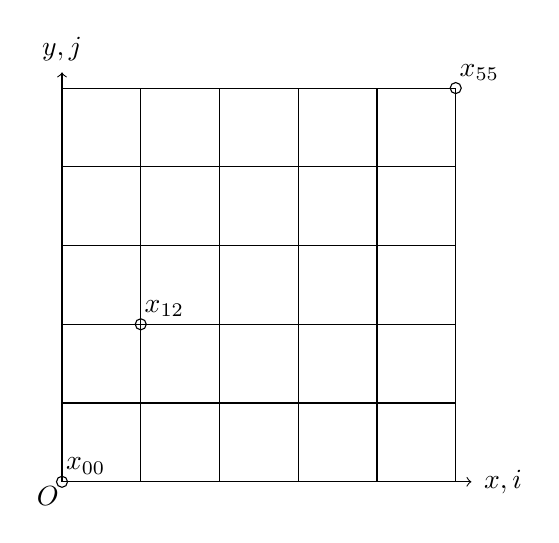
\begin{tikzpicture}
%grid
\draw (0,0) grid +(5,5);

%axes
\draw[->] (0,0) -- (xyz cs:x=0, y=5.2);
\draw (0,5.5) node {$y,j$};

\draw[->] (0,0) -- (xyz cs:x=5.2,y=0);
\draw (5.6,0) node {$x,i$};
\draw (-0.18,-0.18) node {$O$};

\draw (0.3,0.2) node {$x_{00}$};
\draw (0,0) circle (2pt);

\draw (5.3,5.2) node {$x_{55}$};
\draw (5,5) circle (2pt);

\draw (1.3,2.2) node {$x_{12}$};
\draw (1,2) circle (2pt);
\end{tikzpicture}
\caption{Malha padrão para discretizar Laplace e Poisson\label{malha_poisson}}
\end{figure}
Cada cruzamento de linha indica um ponto no domínio, e a equação \ref{laplace_discreta} será aplicada em quase todos estes postos, com exceção dos de fronteira. O valor dos pontos de fronteira deste primeiro problema foi escolhido fixo, utilizando condições de Dirichlet. 

Pelo fato do método ser iterativo, com um \textit{loop} sendo repetido muitas vezes, até a convergência, é natural escolher um método de parada. Isto poderia ser: (1) escolher um tempo limite de execução, (2) ver a diferença entre duas matrizes após uma iteração completa em seus pontos internos, para analisar se a diferença entre elas é desprezível e se indica convergência, ou ainda (3) pode-se calcular os valor da equação de Laplace em cada ponto interno, que seria o melhor a se fazer, e analisar se a equação está dentro de uma faixa de erro desejada. A segunda maneira de se fazer isto foi escolhida na primeira parte, e foi uma difícil decisão escolher qual utilizar, pois ainda não se compreendia como aplicar o terceiro método.

O problema inicialmente proposto tem condições de Dirichlet, que indica a função em cada fronteira do domínio. E os problemas todos são resolvidos num quadrado de lado igual a 1.
\begin{eqnarray}
\nabla^2 u=0 \\
(x,y) \in D\,; 0\le x\le 1\,\textrm{e}\,0\le y\le 1 \nonumber \\
u(0,y)=h_1(y) \nonumber \\
u(1,y)=h_2(y) \nonumber \\
u(x,0)=g_1(x) \nonumber \\
u(x,1)=g_2(x) \nonumber \\
\Delta x = \frac{1}{n-1} \nonumber
\end{eqnarray}

Agora, apresenta-se o algoritmo que se utilizou para resolver a equação
\begin{algorithm}
\SetKwInOut{Input}{input}\SetKwInOut{Output}{output}
\Input{Matriz com as condições de contorno de tamanho $n\times n$}
\Output{Matriz com cada ponto interno satisfazendo a equação de Laplace e a fronteira igual à entrada}
\BlankLine
$STOP=0$\;
$err \leftarrow 10^{-6}$\;
\While{$STOP \neq 1$}{\label{InRes1}
$u^{\textrm{old}}\leftarrow u$\;

\For{$i\leftarrow 1$ \KwTo $n-2$}{
\For{$j\leftarrow 1$ \KwTo $n-2$}{\label{forins}
$u_{ij}\leftarrow (u_{i+1j}+u_{i-1j}+u_{ij+1}+u_{ij-1})/4$\;
}
}
$ERROR\leftarrow Norma(u^{\textrm{old}}-u)$\;

\If{$ERROR < err$}{
$STOP\leftarrow1$\;
}
}

\caption{Resolvendo Laplace Iterativamente}\label{algo_laplace_iter}
\end{algorithm}

Na equação de Laplace, o $\Delta x$ não aparece diretamente, tanto que não aparece no algoritmo, mas esta variável contém um valor importante que será usada nos problemas posteriores de Poisson e Navier Stokes.

O método de resolução apresentado é explícito, no qual o valor de cada ponto no método é obtido diretamente dos pontos adjacentes, e se faz necessária uma resolução iterativa. Isso tem um custo de processamento razoável, no qual o tempo aumenta grandemente conforme o número de pontos $n$ escolhido. Tendo em vista uma resolução mais rápida e direta, pode-se utilizar o método implícito.

Anteriormente, a partir da equação \ref{laplace_discreta_zero}, isolou-se $u_{ij}$ e então resolveu-se iterativamente nosso problema. Outra forma de se resolver o mesmo problema é pegar essa mesma equação e trocar os índices $(i,j)$ por números de fato, obtendo várias equações, e isolando na parte da direita os termos de fronteira. Assim, para um sistema $n\times n$, dos $n^2$ pontos da malha dos índices $(0,0)\rightarrow (n-1,n-1)$, $(n-1)^2$ pontos são internos, correspondendo aos índices de $(1,1)\rightarrow (n-2,n-2)$. A seguir temos as equações para um sistema $5\times 5$:

\begin{eqnarray}
u_{12}+u_{21} -4u_{11}& = & -u_{01}-u_{10} \nonumber \\
u_{11}+u_{22}+u_{31}-4u_{21}& =& -u_{20} \nonumber \\
u_{21}+u_{32}-4u_{31}&=&-u_{41}-u_{30} \nonumber \\
u_{22}+u_{13}+u_{11}-4u_{12}&=&-u_{02} \nonumber \\
u_{32}+u_{12}+u_{23}+u_{21}-4u_{22}&=&0 \nonumber \\
u_{22}+u_{33}+u_{31}-4u_{32}&=&-u_{42} \nonumber \\
u_{23}+u_{12}-4u_{13}&=&-u_{03}-u_{14} \nonumber \\
u_{33}+u_{13}+u_{22}-4u_{23}&=&-u_{24} \nonumber \\
u_{23}+u_{32}-4u_{33}&=&-u_{43}-u_{34} \nonumber
\end{eqnarray}

O conjunto de equações acima é um sistema linear, e é possível representá-lo na forma matricial $Ax = b$. O que torna este problema interessante é que a matriz $A$ e $b$ tem padrões muito bem definidos. A matriz $A$ toma a seguinte forma:
\[ \left( \begin{array}{ccccccccc}
-4 & 1 & 0 & 1 & 0 & 0 & 0 & 0 & 0 \\ % 1
1 & -4 & 1 & 0 & 1 & 0 & 0 & 0 & 0 \\ % 2
0 & 1 & -4 & 0 & 0 & 1 & 0 & 0 & 0 \\ % 3
1 & 0 & 0 & -4 & 1 & 0 & 1 & 0 & 0 \\ % 4
0 & 1 & 0 & 1 & -4 & 1 & 0 & 1 & 0 \\ % 5
0 & 0 & 1 & 0 & 1 & -4 & 0 & 0 & 1 \\ % 6 
0 & 0 & 0 & 1 & 0 & 0 & -4 & 1 & 0 \\ % 7
0 & 0 & 0 & 0 & 1 & 0 & 1 & -4 & 1 \\ % 8
0 & 0 & 0 & 0 & 0 & 1 & 0 & 1 & -4 \\ % 9
\end{array} \right)\]

Observando o padrão de formação da matriz $A$ pentadiagonal e sabendo-se também obter o vetor de valores conhecidos $b$, tem-se um sistema linear para obter os pontos internos $x$. A solução é $x=A^{-1}b$.

Como se nota, a resolução é muito mais direta, mas o algoritmo para se resolver este sistema linear pode ser muito mais complexo. Não se preocupou em criar um algoritmo para isso, mas sim em utilizar um pronto da biblioteca Eigen. Mas há um problema para este método, que um sistema pode ficar extremamente grande com um $n$ relativamente pequeno, tão grande, ao ponto de necessitar de mais memória do que o computador tem. Isso se resolve utilizando matrizes esparsas, que só salvam na memória elementos diferentes de zero. A matriz $A$ é uma matriz esparsa, na qual a maioria de seus elementos é igual a 0. Também utilizaram-se métodos prontos para resolução de sistemas esparsos provenientes da Eigen.
\subsection{Equação de Poisson}

A equação de Poisson é muito similar a de Laplace, mas com uma diferença, que é a de haver uma função forçamento existente no lado direito da equação.
\begin{equation}
  \nabla^2 u=\frac{\partial^2 u}{\partial x^2}+\frac{\partial^2 u}{\partial y^2}=f(x,y)\label{poisson}
\end{equation}

Este foi o segundo problema proposto, e o fato de ter essa função $f(x,y)$ complica o problema porque muita coisa que antes era desconsiderada com o $0$ na equação de Laplace não é mais ignorado, mas sim levado em consideração. No caso explícito, tem-se a seguinte discretização obtida:
\begin{equation}
u_{ij}=\frac{1}{4}[(u_{i+1j}+u_{i-1j}+u_{ij+1}+u_{ij-1})-\Delta x^2 f_{ij}] \label{poisson_discreta}
\end{equation}

O algoritmo iterativo para este caso é o mesmo anterior, substituindo a equação \ref{laplace_discreta} por \ref{poisson_discreta} no algoritmo.

Para o caso implícito, o problema é muito similar, bastando mudar o vetor $b$, que passa a apresentar termos $\Delta x^2 f_{ij}$.
\subsection{Navier Stokes}

Após resolver-se as equações de Laplace e Poisson com condições de Dirichlet, pelos métodos explícito e implícito, tem-se já uma base para partir para a próxima etapa: Navier Stokes. Essa equação tem muitas complicações, e está levando ainda certo tempo para ter-se um programa que a resolva, e esteja de fato livre de bugs. A complexidade do programa é maior, tem muitas etapas, e tem ainda uma evolução no tempo que não foi lidada no problema de Poisson. A equação de Navier Stokes é a seguinte:

\begin{eqnarray}
\rho\left( \frac{\partial \textbf{v}}{\partial
t}+\textbf{v}\cdot\nabla\textbf{v}\right)=-\nabla
p+\mu\nabla^2\textbf{v}+\textbf{f} \label{ns}\\
 \nabla\cdot \textbf{v}=0 \nonumber
\end{eqnarray}

A discretização não é simples e é um pouco diferente da que foi feita anteriormente no problema de Poisson. Primeiramente, tem-se de saber que a discretização de Navier Stokes que será feita aqui é a fórmulação em variáveis primitivas. Isso quer dizer que o problema será trabalhado com as variáveis originais de velocidade $u$, $v$ (em $x$ e $y$) e pressão $p$. Outra forma de resolver é usando uma formulação com a vorticidade, que não será trabalhada aqui.

No que se aprendeu lendo um material em pdf que ensina o processo de resolução em variáveis primitivas, sabe-se que utilizando a malha da Figura \ref{malha_poisson}, ocorre modos espúrios de pressão que causa uma solução de velocidades que contém oscilações não esperadas no resultado do problema. O resultado desta forma não é satisfatório, e para resolver este problema usa-se uma malha escalonada.

A malha escalonada é uma malha na qual um ponto não salva a informação que é exatamente do local onde o ponto se situa, mas de um local próximo. No ponto $P=(i,j)$ são salvos cinco valores: força horizontal, força vertical, pressão, velocidade horizontal e vertical. Essas são representadas pelos símbolos $f_x$, $f_y$, $p$, $u$ e $v$. Um elemento da malha escalonada é representado na figura a seguir, na qual as forças não estão mostradas, mas elas são localizadas nas mesmas posições que as velocidades.

\begin{figure}[!ht]
\centering
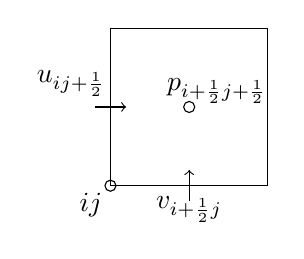
\begin{tikzpicture}
\draw (0,0) rectangle (2,2);
\draw (1.35,1.2) node {$p_{i+\frac{1}{2}j+\frac{1}{2}}$};
\draw[->] (1,-0.2) -- (1,0.2);
\draw (1,-0.3) node {$v_{i+\frac{1}{2}j}$};
\draw[->] (-0.2,1) -- (0.2,1);
\draw (-0.5,1.3) node {$u_{ij+\frac{1}{2}}$};
\draw (1,1) circle (2pt);

\draw (0,0) circle (2pt);
\draw (-0.25,-0.25) node {$ij$};
\end{tikzpicture}
\caption{Elemento de malha escalonada}
\end{figure}

Diferente dos problemas de Laplace e Poisson, no qual um elemento $u_{ij}$ que estava salvo no computador na posição $ij$ realmente é o elemento $u_{ij}$, agora o elemento $u_{ij}$ salvo na memória do computador é fisicamente o elemento $u_{ij+\frac{1}{2}}$, enquanto o elemento $v_{ij}$ se refere ao elemento $v_{i+\frac{1}{2}j}$. De maneira similar ocorre para as forças. Para a pressão, $p_{ij}$ corresponde ao ponto $p_{i+\frac{1}{2}j+\frac{1}{2}}$.


\subsubsection{Desconsiderando a pressão}
A primeira etapa consiste literalmente de desconsiderar a pressão. Há um termo de pressão na equação \ref{ns} que é $\nabla p$. A partir dessa simplificação, faz-se a discretização da equação. Alguns termos foram incluídos nas equações a seguir de forma a tornar algumas das equações menos extensas.
 
\begin{eqnarray}
\textbf{v}_{ij}^s=(u_{i+1j}+u_{i-1j}+u_{ij+1}+u_{ij-1})\textbf{i} 
\nonumber \\+(v_{i+1j}+v_{i-1j}+v_{ij+1}+v_{ij-1})\textbf{j}\\
\textbf{v}_{ij}^t=0.25(u_{ij}+u_{i+1j}+u_{i+1j-1}+u_{ij-1})\textbf{i}\nonumber \\
+0.25(v_{ij}+v_{i-1j}+v_{i-1j+1}+v_{ij+1})\textbf{j}
\end{eqnarray}
\begin{eqnarray}
u_{ij}^{*}&=&\left[\frac{\mu}{\rho}\left(\frac{u_{ij}^s-4u_{ij}}{\Delta
x^2}\right)+\frac{1}{\rho}\frac{f_{x,ij}+f_{x,i-1j}}{2}\right] + u_{ij}\nonumber \\
&-&\left[u_{ij}\frac{u_{i+1j}-u_{i-1j}}{2\Delta
x}-v_{ij}^t\frac{u_{ij+1}-u_{ij-1}}{2\Delta x}\right]\Delta t
\end{eqnarray}

\begin{eqnarray}
v_{ij}^{*}&=&\left[\frac{\mu}{\rho}\left(\frac{v_{ij}^s-4v_{ij}}{\Delta
x^2}\right)+\frac{1}{\rho}\frac{f_{y,ij}+f_{y,ij-1}}{2}\right] + v_{ij}\nonumber \\
&-&\left[u_{ij}^t\frac{v_{i+1j}-v_{i-1j}}{2\Delta
x}-v_{ij}\frac{v_{ij+1}-v_{ij-1}}{2\Delta x}\right]\Delta t
\end{eqnarray}
\section{Resultados}
\subsection{Laplace - Método Iterativo}
Foram realizados vários testes utilizando as seguintes condições:
\begin{eqnarray}
\nabla^2 u=0\\
u_{}
\end{eqnarray}

\section{Conclusão}

% use section* for acknowledgement
\section*{Agradecimentos}

Primeiramente agradeço a Deus pela oportunidade de ter feito parte deste trabalho. Agradeço também ao professor Yuri Dumaresq pelas orientações e ânimo no ensino que eu vi nele e que também me animaram na resolução destes problemas numéricos. Agradeço também ao CNPq pela bolsa de incentivo à pesquisa.

\begin{thebibliography}{4}
  
\bibitem{ubuntu} \href{ftp://ftp.fisio.cinvestav.mx/Manuales/linux/Getting\%20Started\%20with\%20Ubuntu\%2010.10.pdf}{Getting Started with Ubuntu 10.10}
\bibitem{openkinect} \href{http://openkinect.org/wiki/Main_Page}{OpenKinect}
\end{thebibliography}
\end{document}
